% Q8: 按固定候选 PDF 第1页（印刷页282）交通环岛图重绘。
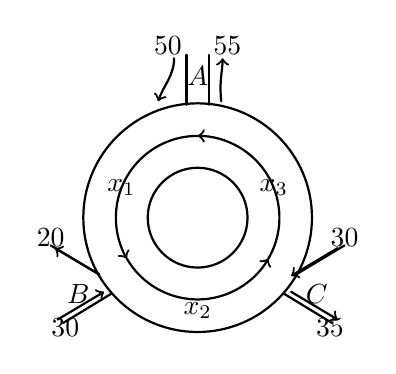
\begin{tikzpicture}[line cap=round,line join=round,scale=0.88]
  % 环岛外缘与中心圆岛
  \draw[thick] (0,0) circle (1.65);
  \draw[thick] (0,0) circle (0.72);

  % 三处外接道路
  \draw[thick] (-0.16,1.63)--(-0.16,2.35);
  \draw[thick] (0.16,1.63)--(0.16,2.35);
  \draw[thick] (-1.42,-0.82)--(-2.12,-0.40);
  \draw[thick] (-1.25,-1.10)--(-1.94,-1.52);
  \draw[thick] (1.42,-0.82)--(2.12,-0.40);
  \draw[thick] (1.25,-1.10)--(1.94,-1.52);

  % 环岛内部方向：A -> B -> C -> A
  \draw[->,thick] (90:1.18) arc (90:210:1.18);
  \draw[->,thick] (210:1.18) arc (210:330:1.18);
  \draw[->,thick] (330:1.18) arc (330:450:1.18);
  \node at (-1.10,0.43) {$x_1$};
  \node at (0,-1.34) {$x_2$};
  \node at (1.10,0.43) {$x_3$};

  % 路口 A：流入 50，流出 55
  \draw[->,thick] (-0.34,2.30) .. controls (-0.34,2.05) and (-0.49,1.91) .. (-0.57,1.68);
  \draw[->,thick] (0.34,1.68) .. controls (0.31,1.98) and (0.36,2.12) .. (0.36,2.30);
  \node at (-0.43,2.48) {$50$};
  \node at (0.43,2.48) {$55$};
  \node[above] at (0,1.76) {$A$};

  % 路口 B：流入 30，流出 20
  \draw[->,thick] (-1.42,-0.82)--(-2.06,-0.44);
  \draw[->,thick] (-2.02,-1.47)--(-1.35,-1.07);
  \node at (-2.12,-0.29) {$20$};
  \node at (-1.91,-1.59) {$30$};
  \node[below left] at (-1.42,-0.82) {$B$};

  % 路口 C：流入 30，流出 35
  \draw[->,thick] (2.02,-0.44)--(1.35,-0.84);
  \draw[->,thick] (1.35,-1.07)--(2.02,-1.47);
  \node at (2.12,-0.29) {$30$};
  \node at (1.91,-1.59) {$35$};
  \node[below right] at (1.42,-0.82) {$C$};
\end{tikzpicture}
